\documentclass[11pt,reqno]{article}
\usepackage{geometry}
\geometry{letterpaper}

\usepackage{graphicx}
\usepackage{amssymb}
\usepackage{amsmath}
\usepackage{tikz}
\usetikzlibrary{arrows,calc,through,intersections,decorations}

\DeclareGraphicsRule{.tif}{png}{.png}{`convert #1 `dirname #1`/`basename #1 .tif`.png}

\title{Sliding down Chords of a Circle}
\author{Satvik Saha}
\date{}
 
\pgfdeclaredecoration{simple line}{initial}{
  \state{initial}[width=\pgfdecoratedpathlength-1sp]{\pgfmoveto{\pgfpointorigin}}
  \state{final}{\pgflineto{\pgfpointorigin}}
}
\tikzset{
   shift left/.style={decorate,decoration={simple line,raise=#1}},
   shift right/.style={decorate,decoration={simple line,raise=-1*#1}},
}

\begin{document}
\maketitle

Points $A$, $B$, $C$ lie on a circle.
A particle at rest at point $A$ falls under the influence of gravity along $AC$, reaching point $C$ in time $t$. The line segment $AC$ is inclined from $AB$, a vertical diameter, by an angle $\alpha$. The following figure illustrates the given problem.

\begin{center}
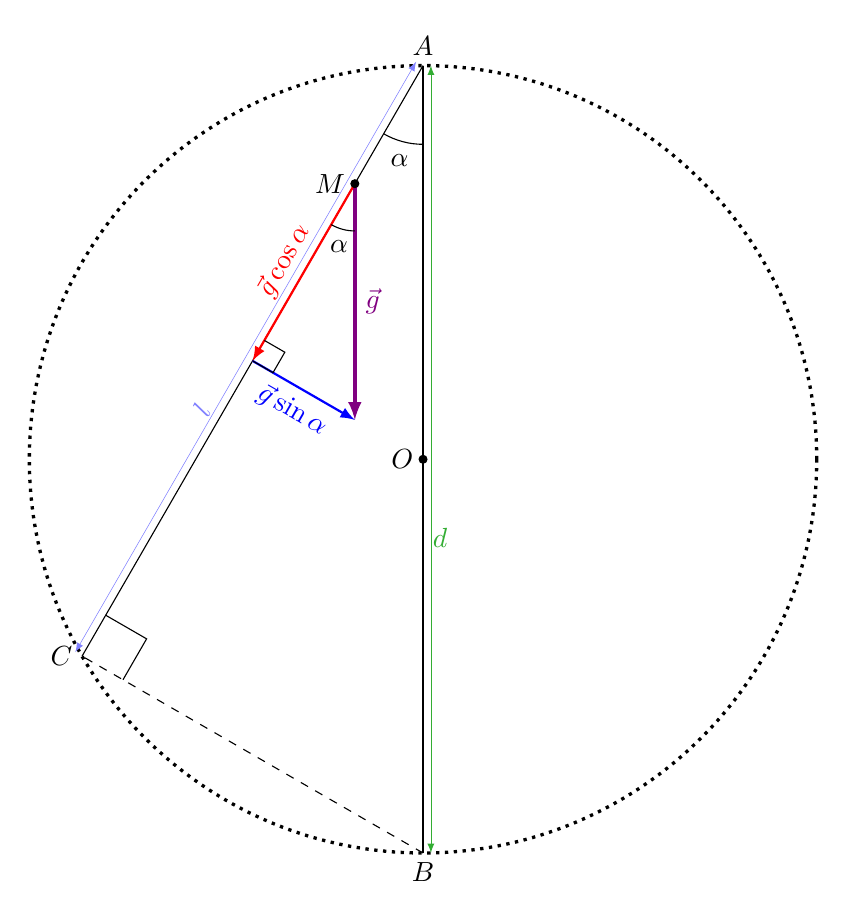
\begin{tikzpicture}
	\coordinate [label=left:$O$]			(O)		at	(0,0);
	\coordinate [label=above:$A$]		(A)		at	(0,5);
	\coordinate [label=below:$B$]		(B)		at	(0,-5);
	\coordinate	[label=left:$C$]			(C)		at	($ (O) + (-150:5) $);
	\coordinate 						(M)		at	($ (A) ! 0.2 ! (C) $);
	\coordinate							(g)		at	($ (M) + (-90:3) $);
	
	\draw[fill=black] (O) circle(0.5mm);
	\node(E) [name path=E,dotted, very thick, draw, circle through=(A)] at (O) {};
	
	\draw (A) -- (B);
	\draw[dashed] (B) -- (C);
	\draw (A) -- (C);
	\draw[rotate=-30] ($ (C) ! 6mm ! (B) $) |- ($ (C) ! 6mm ! (A) $);
	\draw (A) ++ (-90:10mm) arc (-90:-120:10mm);
	\node at ($ (A) + (-3mm, -12mm)$) {$\alpha$};
	
	\draw[-latex, very thick, red!50!blue] (M) -- (g) node[midway, right] {$\vec{g}$};
	\draw[-latex, thick, rotate=-30, blue] (g -| C) -- (g) node[midway, below, rotate=-30] {$\vec{g}\sin\alpha$};
	\draw[-latex, thick, rotate=-30, red] (M) -- (g -| C) node[midway, above, rotate=60] {$\vec{g}\cos\alpha$};
	\draw (M) ++ (-90:6mm) arc (-90:-120:6mm);
	\node at ($ (M) + (-2mm, -8mm)$) {$\alpha$};
	\draw[rotate=-30] (g -| C) -- ($ (g -| C) ! 3mm ! (g) $) |- ($ (g -| C) ! 3mm ! (A) $);
	\draw[fill=black] (M) circle(0.5mm) node[above, left] {$M$};

	\path[<->, >=latex, very thin, blue!50!white] (A) edge[shift right=1mm] (C);
	\path[<->, >=latex, very thin, green!60!black!80] (A) edge[shift left=1mm] (B);
	
	\draw[blue!50!white] ($ (A) ! 0.6 ! (C) $) node[above, rotate=60] {$l$};
	\draw[green!60!black!80] ($ (A) ! 0.6 ! (B) $) node[right] {$d$};
	
\end{tikzpicture}
\end{center}

Note that $\Delta ABC$ is right-angled at $C$. Therefore, we have :

\begin{align*}
	l		\;&=\;	d \,\cos\alpha			\\
	a_{l}	\;&=\;	-g \,\cos\alpha
\end{align*}

Where $a_l$ is the net acceleration of the particle along $AC$.
The equations of uniformly accelerated motion along a straight line along $AC$ give :

\begin{align*}
	-l		\;&=\;	v_0 t	\;+\;	\frac{1}{2}a_lt^2,		\\
	-d\,\cos\alpha	\;&=\;	-\frac{1}{2}\,g\,\cos\alpha\,t^2, \\\\
	t	\;&=\;	\sqrt\frac{2d}{g}
\end{align*}

Clearly, the time taken to reach $C$ from $A$ along a straight line is independent of the angle $\alpha$ made with the vertical. Thus, time taken for a particle to slide from the highest point of a circle down to any other point on the circumference via a chord is a constant.

\end{document}  